%% \chapter[htoc-titlei][hhead-titlei]{htitlei}
%% -----------------------------------------------------------------------------
\chapter[Analysis Summary][Analysis Summary]{Analysis Summary}
\label{chapter:analysis} 

This chapter provides an overview the of analysis searching for SM
production of the Higgs boson in association with top quarks in
multi-lepton final states. The analysis searches in signal regions
with 2 same-sign, 3 and 4 light leptons ($e, \mu$), which are sensitive to Higgs
decays to vector bosons, $H\rightarrow W^{\pm}W^{\pm}$ and $H\rightarrow
Z^{\pm}Z^{\pm}$. We refer to these channels
as 2$\ell$ SS, 3$\ell$, and 4$\ell$ through the rest
of this document. 

The multi-lepton channels form a complement to already completed \tth\ searches in
final states targeting the $H\rightarrow b\bar{b}$ \cite{Aad:2014lma},
$H\rightarrow\gamma\gamma$\cite{ATLAS-CONF-2014-011}. The \tth searches
in the $H\rightarrow\tau\tau$ decay modes were developed concurrently with the
multi-lepton searches, but we do not discuss these here.  
Of this set of complementary searches, the multi-lepton and $b\bar{b}$ are the most sensitve. 

Based on SM production cross-sections, observation lies just outside the sensitivity
of the Run I dataset, even when combining all searches. Instead, the analyses provide an opportunity to 
constrain for the first time the \tth production mode with limits reasonably close to the
actual production rate. The multi-lepton analysis is therefore optimized to overall sensitivity to the 
\tth production rather than individual decay modes, which would be more useful for
constraining Higgs couplings. 

Detailed description of the event and objection section are provided in Chapter \ref{chapter:selection},
background modeling in Chapter \ref{chapter:background}, the effect of systematic errors and the 
statistical analysis in Chapter \ref{chapter:systematics} and final results in Chapter \ref{chapter:results}.


\section{Signal Characteristics} 

\begin{figure}[!t]
\centering
\begin{tabular}{ccc}
\subfloat[2$\ell$ SS]{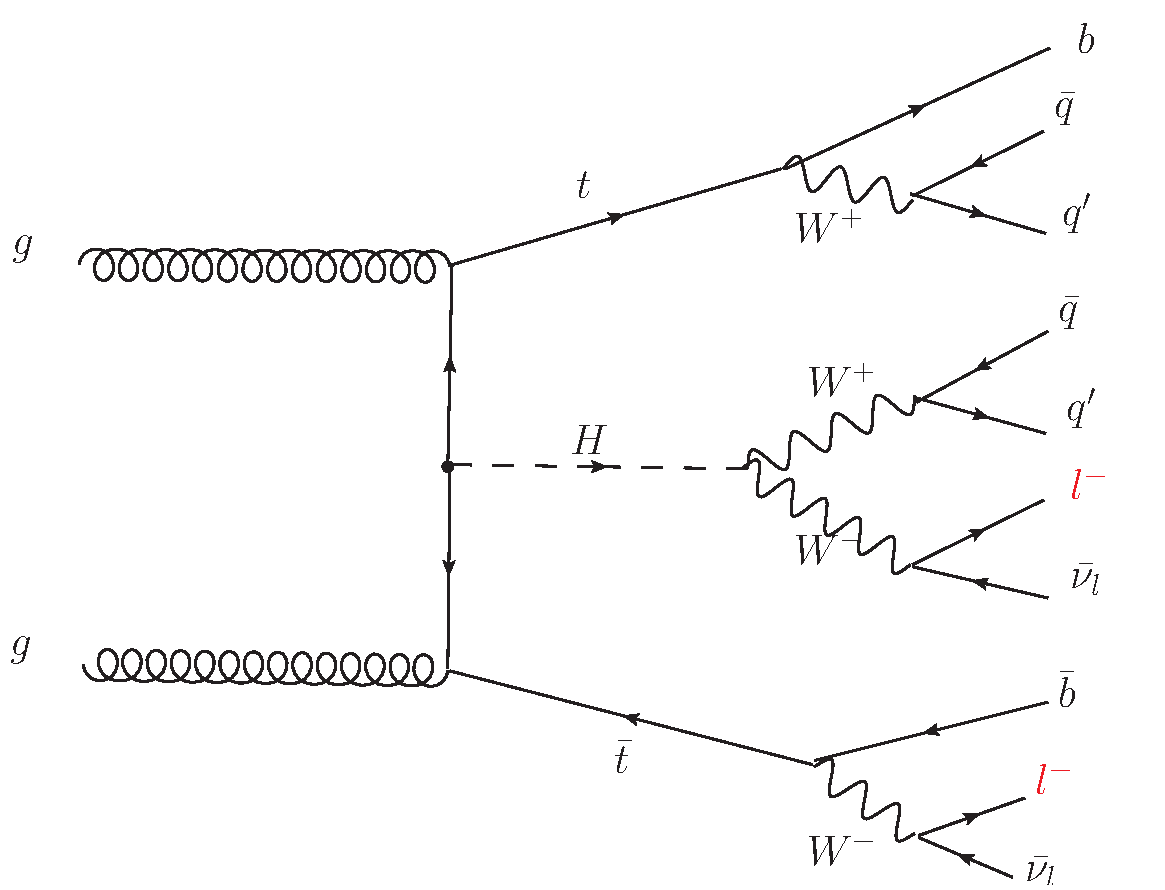
\includegraphics[width=0.30\textwidth]{figs/analysis/2l.pdf}} &
\subfloat[3$\ell$]{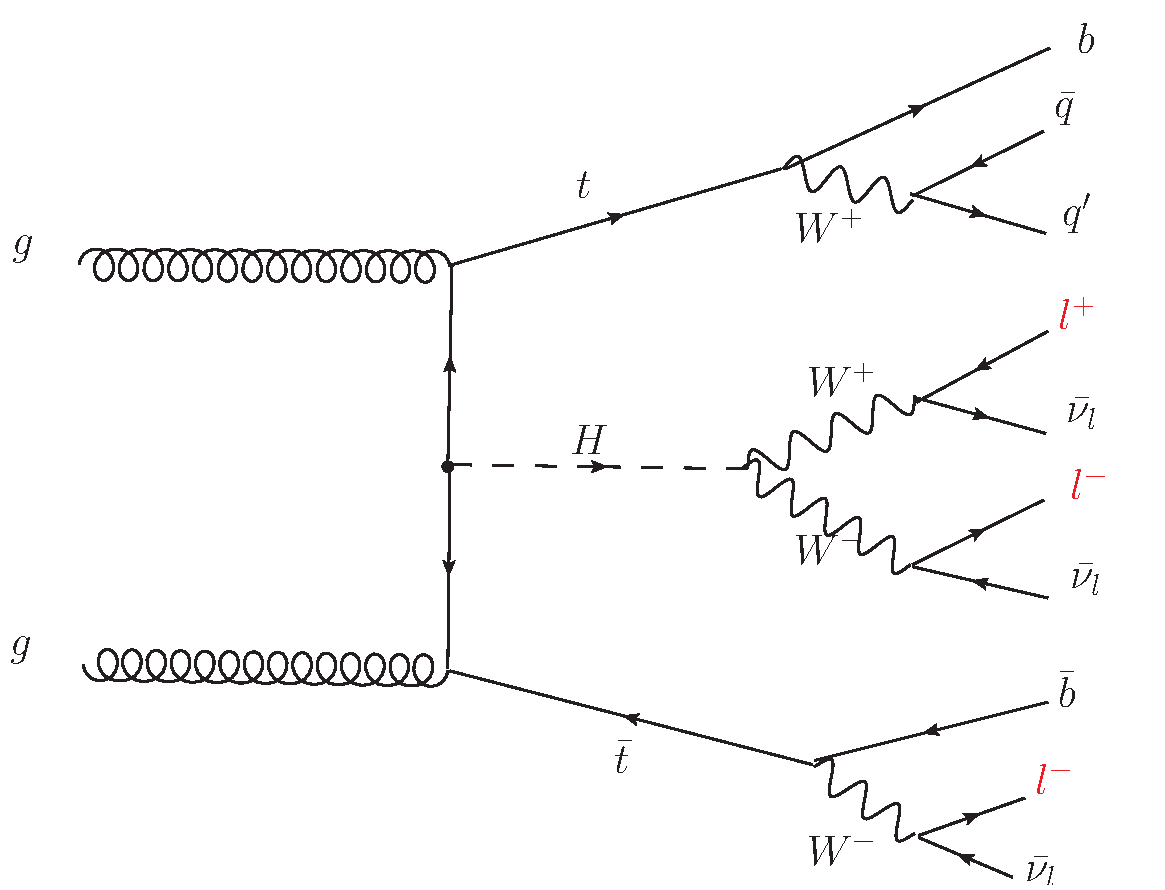
\includegraphics[width=0.30\textwidth]{figs/analysis/3l.pdf}} &
\subfloat[4$\ell$]{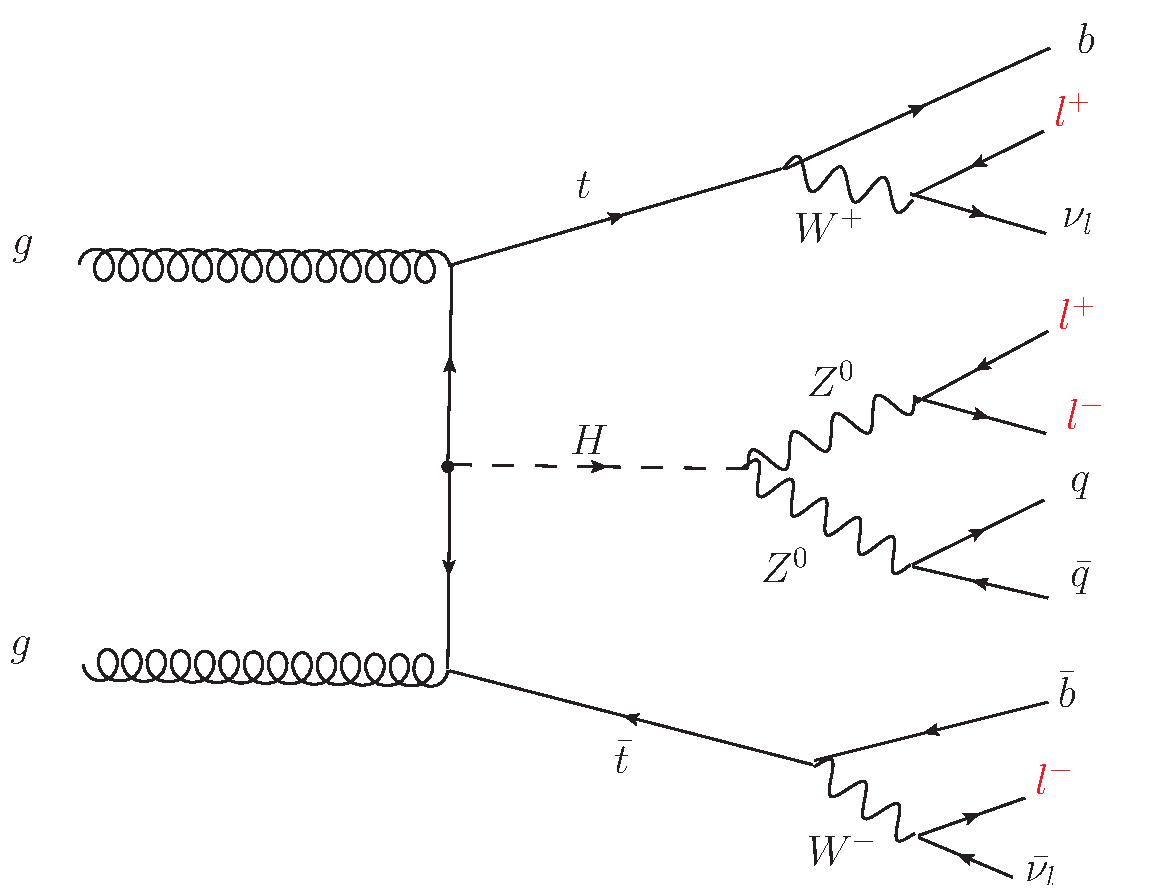
\includegraphics[width=0.30\textwidth]{figs/analysis/4l.pdf}} 
\end{tabular} 
\caption{Example feynman diagrams for the 3 \tth multi-lepton categories.}
\label{figure:ana_diagrams}
\end{figure}

The signal is expected to be characterized by the presence of 2 b-quark jets from
the top quark decays, isolated leptons from vector boson and tau decays,
a high jet multiplicity, and missing energy from neutrionos. Three Higgs boson decays are relevant for this analysis: \WW,
\twotau and \ZZ. All modes are generally dominated by the $WW$ signature, though the 3$\ell$ and 4$\ell$
channels possess some contribution from the$\tau\tau$ and $ZZ$ decays. 
Table \ref{ana:table_decay} provides the fractional contribution of the main 
Higgs decay modes at the generator level to \tth search channels and Figure~\ref{figure:ana_diagrams}
shows example diagrams for each channel. In general, the number of leptons is anti-correlated 
with the number of jets, since a vector boson can either decay leptonically 
or hadronically, such that: 

\begin{itemize}
\item in the 2$\ell$ SS channel, the \tth final state contains 6 quarks\footnote{this does not include additional quarks from radiation}. These events
are then characterized by the largest jet multiplicity.

\item In the 3$\ell$, the \tth final state contains 4 quarks

\item In the 4$\ell$ channel, the \tth final state contains a small number of light
quarks, 0 (\hww case), 2 or 4 (\hzz case).

\end{itemize} 


\begin{table}[htbp]
  \begin{center} 
    \caption{Contributions of the main Higgs decay modes to the 3 multi-lepton
      \tth signatures at generation level.
      }\label{ana:table_decay} 
      \begin{tabular}{l|c|c|c} 
      \hline\hline
  Signature & $H \rightarrow WW$  & $H\rightarrow \tau\tau$  & $H \rightarrow
  ZZ$  \\\hline
  Same-sign &  $100\%$ & -- & -- \\
  3 leptons  &  $71\%$ & $20\%$ & $9\%$ \\
  4 leptons  &  $53\%$ & $30\%$ & $17\%$  \\
     \hline
    \end{tabular}
  \end{center}
\end{table}



\section{Background Overview}

For all channels after selection, the size of the signal is of similar order to the expected size of background.
Background processes can be sorted into two categories:

\begin{itemize}

\item \textbf{Reducible:} These processes cannot lead to a final state compatible with the
  signal signature without a mis-reconstructed object. This category includes
  events with a prompt lepton but with mis-reconstructed charge and events
  with jets that "fake" leptons.  The main backgrounds of this sort are \ttbar\ and \zj. Data-driven techniques are used to measure the rate of these processes and strict object
  selection and used to reduce their rate. 

\item \textbf{Irreducible:} Events which can lead to the same final state as the signal.
 The main background of this category are: \ttV, \WZ, and \ZZ.
 They are modeled using the Monte Carlo simulations. In general,
 these backgrounds are combatted with jet and b-tagged jet requirements. 
 Although the jet multiplicity of \ttV is high, the multiplicity of \tth 
 events is still higher. 

\end{itemize}


\section{Analysis Strategy} 


The analysis search is conducted in 3 channels, based on counting of fully identified
leptons: 2$\ell$ SS, 3$\ell$, and 4$\ell$, with cuts optimized separately for each. We further divide the 2$\ell$ SS into sub channels
based on the number of jets and flavor of the leptons and the 4$\ell$ channel into sub-channels enriched and depleted in OS leptons arising from Z decays. 

This analysis is a counting experiment, meaning that the only quantities signficant to measured result are the event counts in the signal
regions and not the event shapes. The measured background rates, expected signal rates and systematic uncertainties are fed into a Poisson 
model and fit to the observed data. The parameter of interest in the fit and the result of this measurment is, $\mu$, the ratio of the fitted
number of \tth events in the signal regions to expected number of \tth\ events in the signal regions. Since we assume SM branching ratios,
$\mu$ can be considered the ratio of the measured \tth\ cross-section to the observed \tth\ cross-section, and we the fitted $\mu$ to be
close to 1 with large statistical errors.

We express the final result as a measurment of $\mu$ with uncertaintites and 95\% upper limit on the value of $\mu$: $\mu$-values higher than this
value will be considered excluded. We provide these results for each channel individually and combined.  




